\chapter{Proposed Methodology}
\label{ch:methodology}

This chapter details the engineering methodology and empirical research procedures proposed to build and evaluate Dawa Lens. It outlines the research design, presents the multi-tiered system architecture, specifies the iterative development lifecycle, and describes data collection and requirements elicitation protocols. Furthermore, the chapter articulates functional and non-functional specifications, development tools, testing protocols, and ethical safeguards.

\section{Research Design}

This project adopts an \textbf{Applied Engineering Design Science Research (DSR)} methodology \cite{hevner2004design}, structured across six sequential phases: (1)~\textbf{Problem Identification}, delineating outpatient adherence barriers in Uganda via clinical guidelines and stakeholder reviews; (2)~\textbf{Solution Objectives}, establishing quantitative engineering metrics (sub-second offline launch latency, $\ge 95\%$ OCR character accuracy, and 100\% offline schedule availability); (3)~\textbf{Artifact Design and Development}, architecting edge computer vision, local IndexedDB persistence, deterministic alarms, and localized food-drug interaction logic; (4)~\textbf{Demonstration}, deploying laboratory testbeds simulating intermittent cellular connectivity and low-cost smartphone constraints; (5)~\textbf{Empirical Evaluation}, measuring technical benchmarks (CER, trigger latency) and conducting a 2-week field pilot ($N=50$) using the standardized System Usability Scale (SUS); and (6)~\textbf{Communication}, documenting contributions in this proposal and the final thesis at Soroti University.

\section{System Architecture}
\label{sec:architecture}

The proposed architecture of Dawa Lens follows an offline-first, edge-native model minimizing cloud dependency. Figure~\ref{fig:architecture} illustrates the four operational tiers:

\begin{figure}[!htbp]
  \centering
  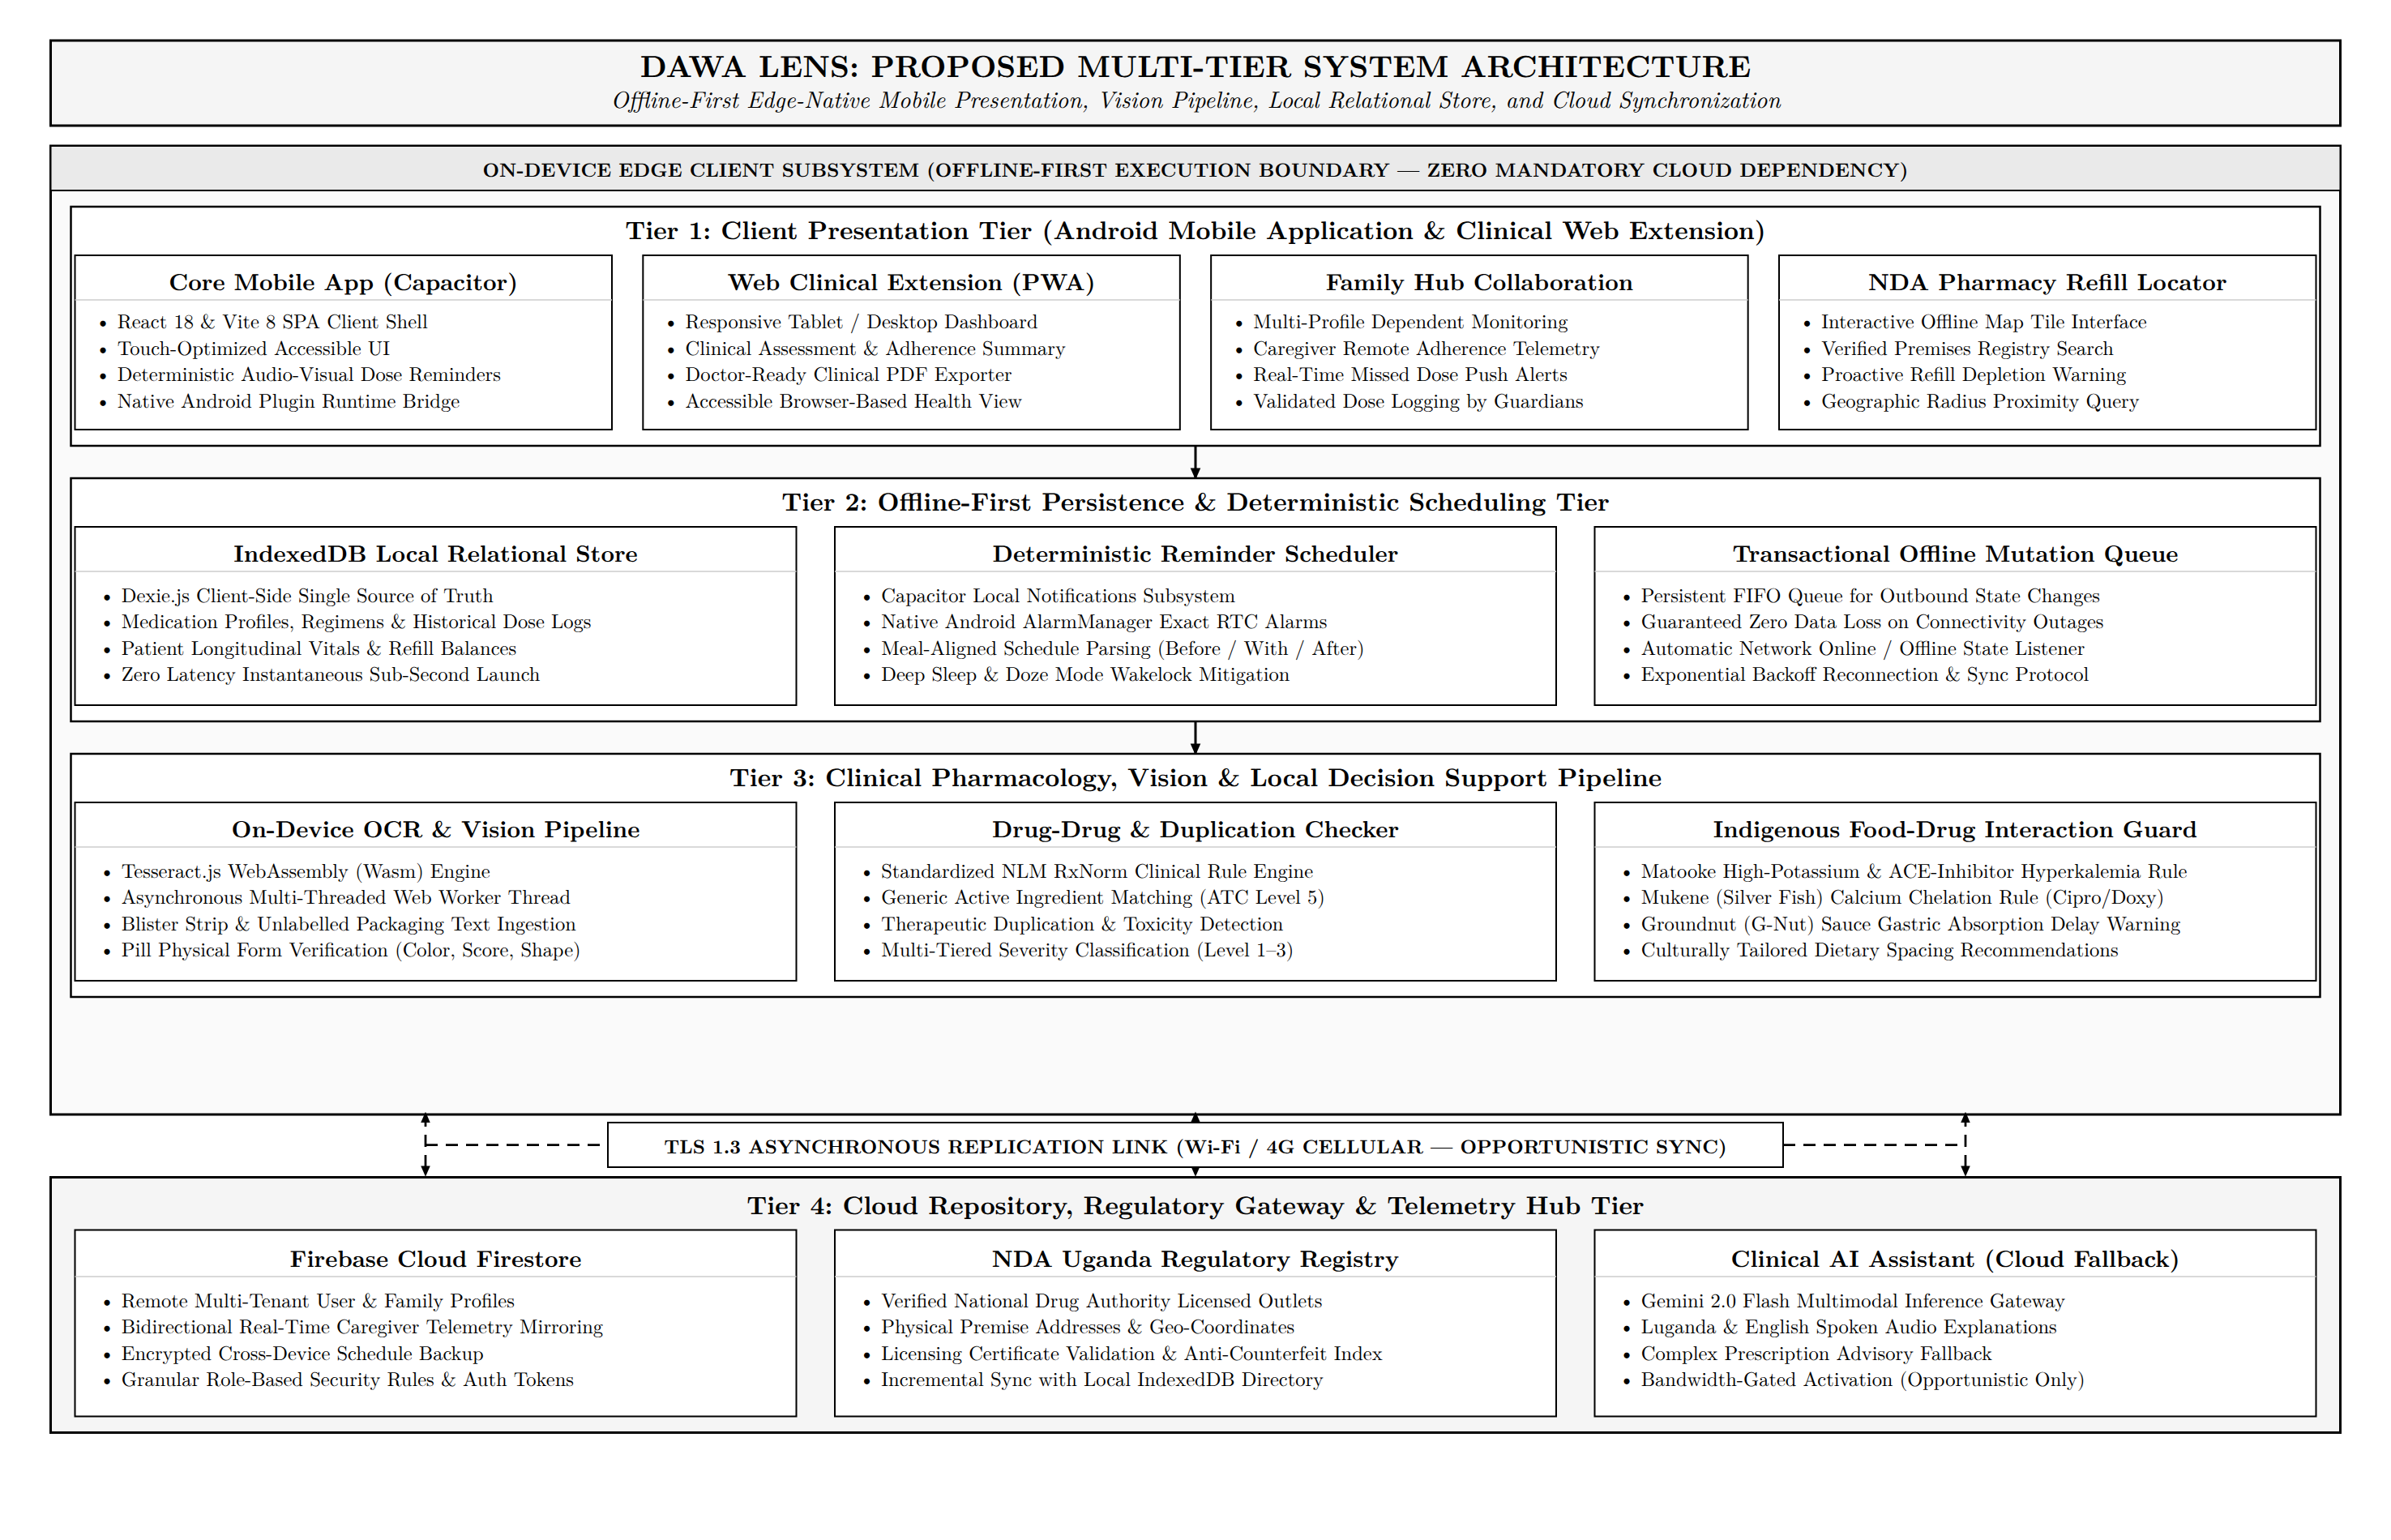
\includegraphics[width=0.95\textwidth,keepaspectratio]{figures/system_architecture.png}
  \caption{Proposed system architecture and hardware-software interconnections of Dawa Lens.}
  \label{fig:architecture}
\end{figure}

\begin{itemize}[noitemsep,topsep=2pt]
  \item \textbf{Tier 1: Client Presentation Tier:} Implemented in React 18, Vite 8, and TypeScript, packaged for Android via Capacitor 8. It encompasses the core mobile touch UI, a responsive Progressive Web App (PWA) extension for clinical PDF export, a Family Hub caregiver interface, and an interactive NDA licensed pharmacy locator.
  \item \textbf{Tier 2: Offline-First Persistence \& Scheduling Tier:} Employs browser-standard IndexedDB (via Dexie.js) as the local source of truth. A deterministic scheduler uses native exact alarm APIs (\texttt{SCHEDULE\_EXACT\_ALARM}) for reliable offline alerting, while an offline FIFO mutation queue buffers local edits with exponential-backoff retry.
  \item \textbf{Tier 3: Clinical Pharmacology \& Vision Pipeline Tier:} Executes Tesseract.js compiled to WebAssembly (Wasm) inside an asynchronous Web Worker to extract packaging text on-device. An inference engine checks active ingredients against RxNorm contraindications and screens indigenous food interactions (\textit{Matooke} and \textit{Mukene}).
  \item \textbf{Tier 4: Cloud Repository \& Regulatory Gateway Tier:} Uses Firebase Cloud Firestore for cross-device caregiver replication, hosts the verified National Drug Authority (NDA) pharmacy registry, and provides an optional Gemini 2.0 Flash fallback for Luganda voice synthesis when bandwidth permits.
\end{itemize}

\section{Development Lifecycle and Requirements Elicitation}

Software development follows an \textbf{Iterative Agile/Prototyping} lifecycle across five two-week sprints: Sprint~1 (Architecture \& IndexedDB setup), Sprint~2 (Deterministic alarm scheduler), Sprint~3 (Edge Wasm OCR pipeline), Sprint~4 (Clinical food-drug matrix \& NDA directory), and Sprint~5 (Family Hub sync, PWA PDF export, and integration testing).

Requirements are elicited through: (1)~\textbf{Document Review} of the \textit{Uganda Clinical Guidelines 2023} \cite{moh2023guidelines}, the \textit{NDA Register of Licensed Drug Outlets} \cite{nda2024register}, and FAO Eastern Africa Food Tables \cite{fao2019food}; (2)~\textbf{Stakeholder Consultations} in Eastern Uganda with community pharmacists ($N=6$) and chronic disease outpatients ($N=10$) in Soroti Municipality; and (3)~\textbf{Technical Profiling} of entry-tier smartphones (Transsion Tecno and Infinix series) to quantify memory limits and camera constraints. System datasets are compiled from NLM RxNorm \cite{rxnorm2024}, the NDA register \cite{nda2024register}, and FAO nutrition tables \cite{fao2019food}.

\section{Tools, Materials and Technologies}

Table~\ref{tab:tools_technologies} enumerates the development stack, test devices, and software frameworks utilized.

\begin{table}[!htbp]
  \centering
  \caption{Engineering tools, hardware materials, and software frameworks.}
  \label{tab:tools_technologies}
  \footnotesize
  \setlength{\tabcolsep}{3.5pt}
  \begin{tabularx}{\textwidth}{@{} >{\raggedright\arraybackslash}p{2.6cm} >{\raggedright\arraybackslash}p{3.8cm} >{\raggedright\arraybackslash}X @{}}
    \toprule
    \textbf{Category} & \textbf{Tool / Technology} & \textbf{Engineering Purpose / Justification} \\
    \midrule
    \textbf{Workstation} & Linux (Ubuntu 24.04 LTS), 16GB RAM, Core i7 & Primary development environment for software implementation and local testing. \\
    \textbf{Test Handsets} & Tecno Spark (Android 11), Samsung Galaxy A-series (Android 14) & Representative real-world test devices reflecting entry-tier and mid-tier handsets in Uganda. \\
    \textbf{Frontend} & React 18, Vite 8, TypeScript & Component-based client architecture providing type safety and rapid rendering. \\
    \textbf{Mobile Runtime} & Capacitor 8 Core & Native bridge providing access to device hardware, local filesystem, and system notifications. \\
    \textbf{Local Datastore} & IndexedDB via Dexie.js & Transactional client-side database for durable offline storage. \\
    \textbf{Computer Vision} & Tesseract.js (Wasm / Web Worker) & Edge-compatible OCR executing client-side without cloud API reliance. \\
    \textbf{Cloud Services} & Firebase Firestore, Firebase Auth & Scalable cloud database, user authentication, and encrypted backup. \\
    \textbf{Styling \& UI} & Tailwind CSS, Lucide Icons & Responsive, utility-first styling ensuring touch accessibility. \\
    \textbf{Testing Suites} & Vitest, Playwright, Chrome DevTools & Unit testing, end-to-end integration testing, and performance profiling. \\
    \bottomrule
  \end{tabularx}
\end{table}

\section{Data Analysis Methods}

Empirical evaluation data collected during laboratory benchmarking and user field trials will be processed across four primary dimensions:
\begin{enumerate}[noitemsep,topsep=2pt]
  \item \textbf{OCR Text Recognition Accuracy:} Character Error Rate $\text{CER} = (S + D + I) / N$ \cite{smith2007tesseract}, targeting $\text{CER} < 5\%$ and clinical entity extraction success $\ge 90\%$.
  \item \textbf{Reminder Timing Fidelity:} Scheduling latency delta across Android background execution and battery-optimizing Doze states \cite{android2024doze} ($|t_{\text{triggered}} - t_{\text{scheduled}}| \le 1.0\,\text{s}$).
  \item \textbf{Usability and Acceptance:} Standardized SUS scores \cite{brooke1996sus} across $N=50$ participants evaluated against Bangor's acceptability benchmarks ($\ge 75/100$) \cite{bangor2008empirical}.
  \item \textbf{Adherence Compliance:} Paired two-tailed $t$-tests ($\alpha = 0.05$) analyzing compliance gains between baseline recall and app-logged data.
\end{enumerate}

\section{Preliminary Requirements and Specifications}

System requirements are partitioned into Functional Requirements (Table~\ref{tab:functional_requirements}) and Non-Functional Requirements (Table~\ref{tab:non_functional_requirements}), mapped to project objectives. Figure~\ref{fig:use_case} visualizes the multi-actor UML use case diagram defining actor boundaries, subsystem roles, and operational dependencies across outpatients, treatment guardians, attending clinicians, and community pharmacists.

\begin{figure}[!htbp]
  \centering
  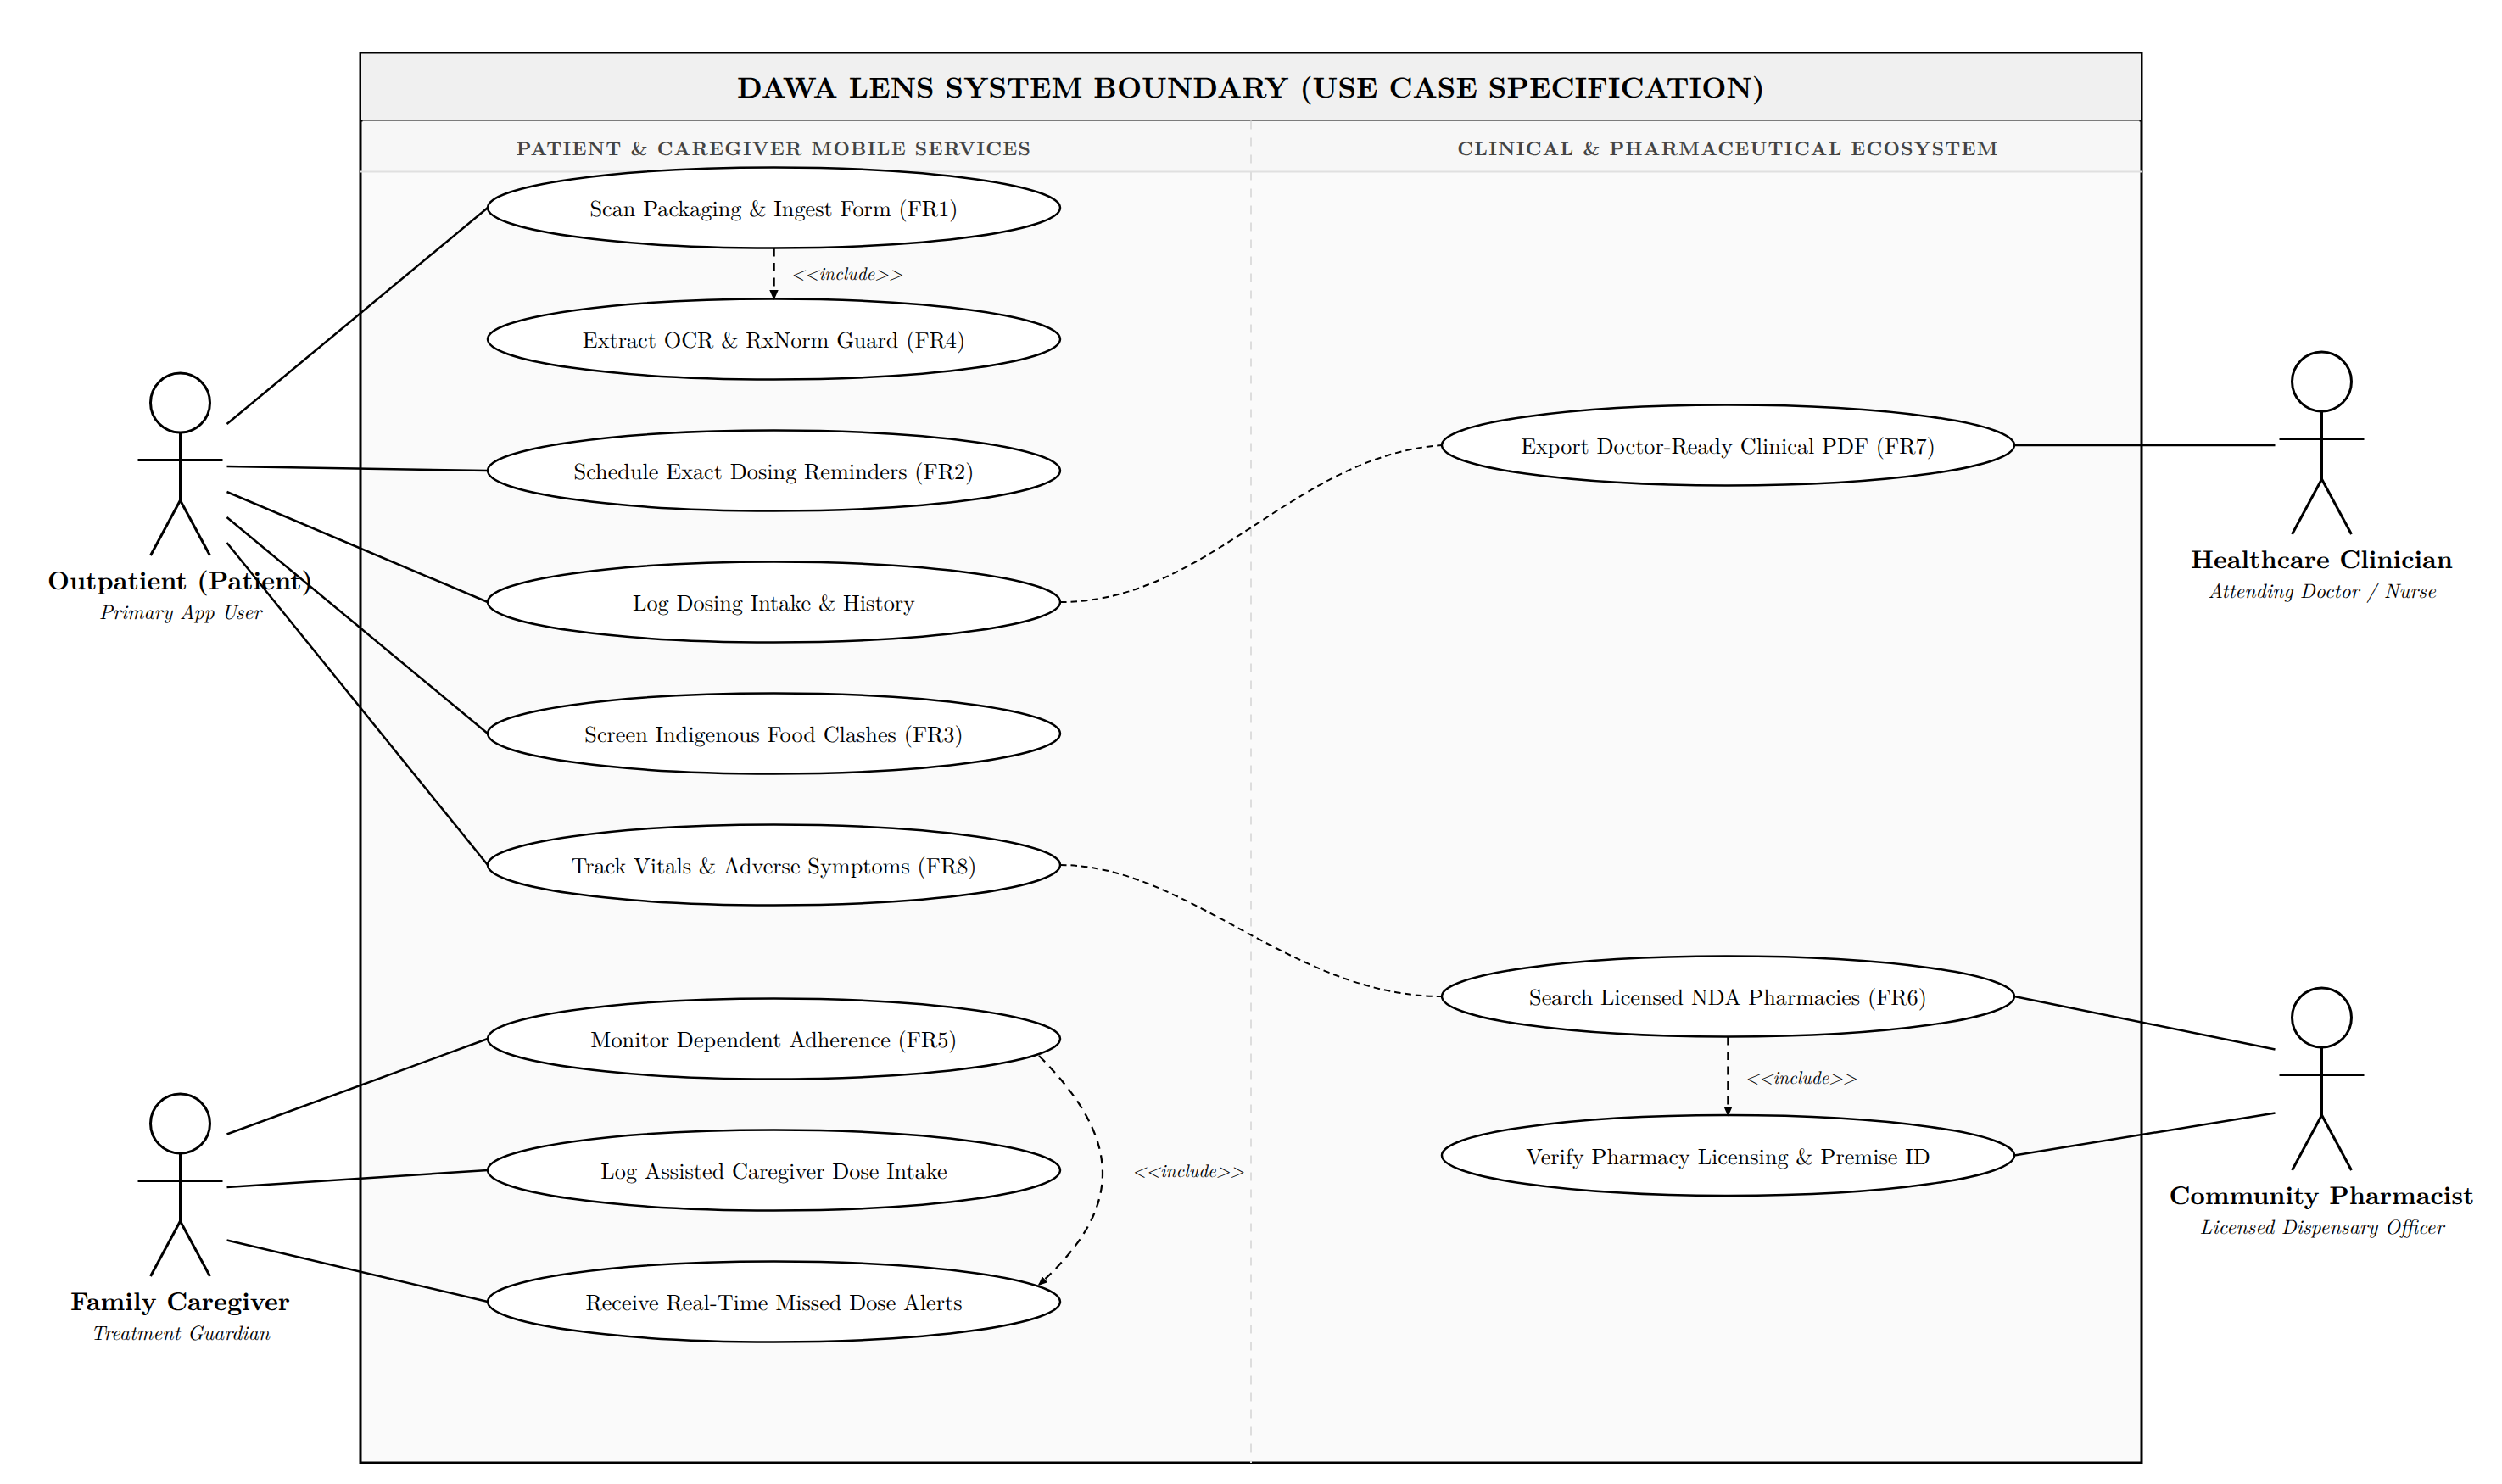
\includegraphics[width=0.95\textwidth,keepaspectratio]{figures/use_case_diagram.png}
  \caption{Multi-actor UML use case specification diagram of the Dawa Lens mobile ecosystem.}
  \label{fig:use_case}
\end{figure}

\begin{table}[!htbp]
  \centering
  \caption{Functional requirements specification and traceability matrix.}
  \label{tab:functional_requirements}
  \scriptsize
  \setlength{\tabcolsep}{3pt}
  \begin{tabularx}{\textwidth}{@{} l >{\raggedright\arraybackslash}p{2.6cm} >{\raggedright\arraybackslash}X >{\raggedright\arraybackslash}p{1.7cm} >{\centering\arraybackslash}p{1.2cm} >{\centering\arraybackslash}p{1.3cm} @{}}
    \toprule
    \textbf{Req ID} & \textbf{Requirement Title} & \textbf{The System Shall...} & \textbf{Primary Actor} & \textbf{Target Obj.} & \textbf{Priority} \\
    \midrule
    \textbf{FR1} & Automated Packaging Scanning & Capture blister packaging images and extract drug identity and dosage parameters using on-device Wasm OCR. & Patient & Obj.~(ii) & Must Have \\
    \midrule
    \textbf{FR2} & Deterministic Offline Schedule & Support interval, time-specific, and meal-aligned dosing schedules stored in local persistence. & Patient & Obj.~(iii) & Must Have \\
    \midrule
    \textbf{FR3} & Indigenous Food-Drug Screener & Screen active drugs against biochemical profiles of Ugandan staples (\textit{Matooke}, \textit{Mukene}) and issue graded warnings. & Patient & Obj.~(iii) & Must Have \\
    \midrule
    \textbf{FR4} & Drug-Drug \& Duplication Guard & Cross-reference RxNorm nomenclatures to detect adverse drug interactions and duplicate active chemicals. & Patient & Obj.~(i), (iii) & Must Have \\
    \midrule
    \textbf{FR5} & Family Caregiver Telemetry Hub & Allow primary caregivers to link dependent profiles, monitor adherence logs, and record assisted doses. & Caregiver & Obj.~(iv) & Must Have \\
    \midrule
    \textbf{FR6} & NDA Licensed Pharmacy Locator & Display geospatial maps and directories of verified community pharmacies licensed by the NDA. & Patient & Obj.~(i), (iv) & Should Have \\
    \midrule
    \textbf{FR7} & Clinical PDF Report Generator & Export longitudinal adherence percentages, missed dose records, and logged vitals as standardized PDF summaries. & Clinician & Obj.~(iv) & Should Have \\
    \midrule
    \textbf{FR8} & Health Metrics Journal & Enable logging of physiological vitals (blood pressure, blood glucose) and self-reported adverse symptoms. & Patient & Obj.~(iii) & Could Have \\
    \bottomrule
  \end{tabularx}
\end{table}

\begin{table}[!htbp]
  \centering
  \caption{Non-functional requirements specification and validation criteria.}
  \label{tab:non_functional_requirements}
  \scriptsize
  \setlength{\tabcolsep}{3pt}
  \begin{tabularx}{\textwidth}{@{} l >{\raggedright\arraybackslash}p{2.2cm} >{\raggedright\arraybackslash}X >{\raggedright\arraybackslash}p{2.4cm} >{\raggedright\arraybackslash}p{2.2cm} @{}}
    \toprule
    \textbf{Req ID} & \textbf{Quality Attribute} & \textbf{Engineering Specification / Constraint} & \textbf{Target Metric} & \textbf{Validation Method} \\
    \midrule
    \textbf{NFR1} & Offline Availability & Core scheduling, alarms, dose logging, and food screening must operate with 0\% network dependence. & 100\% offline availability & Disconnected sandbox testing \\
    \midrule
    \textbf{NFR2} & Execution Latency & Local database queries and edge OCR packaging parsing must execute without UI thread freeze. & OCR $< 2.5\,\text{s}$, DB $< 50\,\text{ms}$ & Chrome DevTools \& Android profiler \\
    \midrule
    \textbf{NFR3} & Alarm Reliability & Scheduled dose reminder alarms must fire accurately at the designated time across Doze states. & $\ge 99.5\%$ on-time trigger fidelity & Automated timing log delta analysis \\
    \midrule
    \textbf{NFR4} & System Usability & Interface must be accessible to users with low literacy, featuring high contrast and intuitive touch targets. & SUS Score $\ge 75/100$ & Standardized SUS field survey ($N=50$) \\
    \midrule
    \textbf{NFR5} & Hardware Efficiency & Background reminder scheduling and local queue processes must minimize battery drain on budget devices. & $< 3\%$ battery drain per 24 hours & Android Battery Historian benchmark \\
    \midrule
    \textbf{NFR6} & Security \& Privacy & Local health records isolated in sandboxed storage, with cloud synchronization encrypted via TLS 1.3. & Zero unencrypted plaintext transmission & Network packet inspection (Wireshark) \\
    \bottomrule
  \end{tabularx}
\end{table}

\section{Testing Strategy and Risk Analysis}

The system will undergo multi-tier verification: automated Vitest unit testing, Playwright integration testing, edge stress testing under network blackouts, and a 2-week field usability evaluation with $N=50$ participants (35 outpatients, 10 caregivers, 5 pharmacists). Table~\ref{tab:test_verification_matrix} formalizes the testing matrix, while Table~\ref{tab:risks} provides the project risk register.

\begin{table}[!htbp]
  \centering
  \caption{Multi-tier testing, verification, and validation matrix.}
  \label{tab:test_verification_matrix}
  \scriptsize
  \setlength{\tabcolsep}{3pt}
  \begin{tabularx}{\textwidth}{@{} l >{\raggedright\arraybackslash}p{2.0cm} >{\raggedright\arraybackslash}p{2.8cm} >{\raggedright\arraybackslash}X >{\centering\arraybackslash}p{1.8cm} @{}}
    \toprule
    \textbf{Test Tier} & \textbf{Subsystem Tested} & \textbf{Test Scenario / Input} & \textbf{Expected Engineering Behavior} & \textbf{Pass Metric} \\
    \midrule
    \textbf{Unit Test} & Recurrence Engine & Leap-year, timezone shift, irregular interval dosing & Deterministic computation of next dosing epoch timestamp & 100\% pass (Vitest) \\
    \midrule
    \textbf{Unit Test} & Food Interaction Guard & Co-ingestion: Enalapril + Matooke, Ciprofloxacin + Mukene & Automated trigger of Level 3 contraindication warning alert & 100\% rule recall \\
    \midrule
    \textbf{Integration} & Offline Mutation Queue & Create reminder $\to$ airplane mode $\to$ log 5 doses $\to$ reconnect & Zero data loss, with ordered FIFO flush to Firestore with retry backoff & 0\% drop rate \\
    \midrule
    \textbf{Edge Stress} & Wasm Packaging OCR & 100 degraded/curved blister foils under low ambient light ($<50\,\text{lux}$) & Binarization filter enhancement; drug name and strength parsed & CER $< 5.0\%$, latency $<2.5\,\text{s}$ \\
    \midrule
    \textbf{Edge Stress} & Local Notification Daemon & Device in Android deep Doze standby for 6 continuous hours & Exact alarm wakes CPU partial lock, and audio-visual alert fires & Trigger delta $\Delta t \le 1.0\,\text{s}$ \\
    \midrule
    \textbf{Field Pilot} & End-to-End System & 2-week continuous outpatient deployment across $N=50$ users & Longitudinal dose logging and weekly PDF report generation & SUS Score $\ge 75/100$ \\
    \bottomrule
  \end{tabularx}
\end{table}

\begin{table}[!htbp]
  \centering
  \caption{Project risk analysis and mitigation register.}
  \label{tab:risks}
  \footnotesize
  \setlength{\tabcolsep}{3.5pt}
  \begin{tabularx}{\textwidth}{@{} >{\raggedright\arraybackslash}p{2.8cm} >{\centering\arraybackslash}p{1.4cm} >{\centering\arraybackslash}p{1.3cm} >{\raggedright\arraybackslash}X @{}}
    \toprule
    \textbf{Identified Risk} & \textbf{Likelihood} & \textbf{Impact} & \textbf{Engineering Mitigation Strategy} \\
    \midrule
    \textbf{OCR Failure on Damaged Foil} & Medium & High & Implement fallback manual search with auto-suggest formulary lookup, allowing user editing of extracted OCR fields. \\
    \midrule
    \textbf{OS Background Alarm Throttling} & Medium & High & Utilize platform exact alarm permissions (\texttt{SCHEDULE\_EXACT\_ALARM}) and persistent local notification channels. \\
    \midrule
    \textbf{Intermittent Cellular Connectivity} & High & Medium & Enforce offline-first architecture with local IndexedDB persistence and transactional FIFO mutation queues. \\
    \midrule
    \textbf{Participant Attrition in Pilot} & Medium & Medium & Recruit an oversampled cohort ($N=60$) to ensure target sample size ($N=50$) is achieved, with airtime stipends provided. \\
    \midrule
    \textbf{Incomplete Local Food Data} & Low & High & Scope food rules to prominent, scientifically verified staples (\textit{Matooke}, \textit{Mukene}, \textit{G-nut sauce}) validated by clinical pharmacists. \\
    \midrule
    \textbf{Scope Creep Delaying Submission} & Medium & High & Adhere strictly to 5-sprint Agile plan, prioritizing core mobile reminder app before secondary web extensions. \\
    \bottomrule
  \end{tabularx}
\end{table}

\section{Ethical Considerations and Chapter Summary}

The study follows strict ethical procedures: written informed consent from all participants, complete anonymization of telemetry, and permanent software disclaimers stating that algorithmic alerts do not replace professional medical advice. Socially, the project advances digital inclusion, combats unregistered drug outlets via NDA registry integration, and eliminates subscription fees. Together, these methodological components establish a disciplined engineering roadmap for executing Dawa Lens at Soroti University.
